\documentclass[a4paper, 10pt]{article}
% import packages
\usepackage[margin=0.2cm]{geometry}
\usepackage{pdflscape}
\usepackage{array}
\usepackage{makecell}
\usepackage{xcolor}
\usepackage{colortbl}
\usepackage{longtable}
\usepackage{titlesec}
\usepackage{float}
\usepackage{needspace}
\usepackage{graphicx}
\usepackage{hyperref}
\usepackage{setspace}
\usepackage{fancyhdr}
\usepackage{enumitem}
\usepackage{multicol}
\usepackage{amsmath}
\usepackage{graphicx}
\usepackage[table]{xcolor}
\usepackage{booktabs}   % for \toprule, \midrule, \bottomrule
\usepackage{adjustbox}  % for \begin{adjustbox}{max width=\textwidth}
\usepackage{etoolbox}
\usepackage{tikz}
\usepackage{caption}
\usepackage{pgfplots}
\pgfplotsset{compat=1.18}
\usepgfplotslibrary{groupplots}
\usetikzlibrary{arrows.meta, positioning, shapes.geometric,fit,calc}

\AtBeginEnvironment{tabular}{\tiny}
\definecolor{cDark}{HTML}{203F4A}
\definecolor{cTeal}{HTML}{1D8F7E}
\definecolor{cGold}{HTML}{E9C06A}
\definecolor{cOrange}{HTML}{F29B5C}
\definecolor{cRed}{HTML}{E85D47}

\renewcommand{\familydefault}{\sfdefault}

\newlength\tindent
\setlength{\tindent}{\parindent}
\setlength{\parindent}{0pt}
\renewcommand{\indent}{\hspace*{\tindent}}

% global list spacing (affects all levels)
\setlist{noitemsep, topsep=0pt, parsep=0pt, partopsep=0pt}


% now explicitly override indentation for each level you care about:
\setlist[itemize,1]{leftmargin=1.2em,label=\raisebox{0.5ex}{\scalebox{0.6}{$\bullet$}}}
\setlist[itemize,2]{leftmargin=1.4em}
\setlist[itemize,3]{leftmargin=0.5em,label=\raisebox{0.5ex}{\scalebox{0.6}{$\bullet$}}}


\setlist[enumerate,1]{leftmargin=1.2em}
\setlist[enumerate,2]{leftmargin=1.4em}
\setlist[enumerate,3]{leftmargin=0.5em}

\setlength{\columnseprule}{0.1pt}
% ------------------------------------------------------


% Configure makecell package
\renewcommand{\theadalign}{bc}
\renewcommand{\theadgape}{\Gape[4pt]}
\renewcommand{\cellgape}{\Gape[4pt]}
\renewcommand{\cellalign}{lt}

% global line spacing
\renewcommand{\baselinestretch}{1.2}

% colour definitions
\definecolor{lightergray}{gray}{0.90}

\providecommand{\tightlist}{%
\setlength{\itemsep}{0pt}
\setlength{\parskip}{0pt}}

\begin{document}
  \begin{landscape}

  
\begin{multicols}{4}

\scriptsize

{\footnotesize{\textbf{ML}}}

\begin{itemize}
    \item Modell
    \begin{itemize}
        \item Wenn für Menschen Intelligent wirkt ist KI auch wenn nicht unbedingt ML
        \item Ausprogrammiert von experten
        \item Wenn Modell gelernt aus Daten \(\rightarrow\) dann ist ML
    \end{itemize}
    \item Learning: Wissen kommt von Experten und/oder Daten
    \item Wissen
    \begin{itemize}
        \item Viel annahmen wenig daten \(\rightarrow\) viel wissen
        \item mittel wissen, mittel daten \(\rightarrow\) mischung ausgewogen
        \item wenig annahmen, viel daten \(\rightarrow\) praktisch alles daten (big player)
    \end{itemize}
    \item Lernphase: Online / Offline \(\rightarrow\) Anwendungsphase
    \item Wie? Supervised, Unsupervised, Reinforced Learning, In-Context Learning
    \item Input (unabhängige Variabel \(\rightarrow\) Output (abhängige Variabel)
\end{itemize}

\vspace{0.4em}
\hrule
\vspace{0.7em}

{\scriptsize{Linear Regression}} Supervised Regression
  \begin{itemize}
    \item \textbf{Input / Output:} Kontinuierlich
    \item \textbf{Annahme}
    \begin{itemize}
        \item 1 Lösung weil Ableitung 0
        \item Lineare Funktion
    \end{itemize}
    \item Wir haben breite von Fisch, wollen das gewicht. Formel ist unveränderlich
    \item \textbf{Data Specification}
    \begin{itemize}
        \item Zielvariabel festlegen
        \item features selection
        \item Encoding Kategorisch
        \item Standardising Nummerisch
    \end{itemize}
    \item \textbf{Model}
    \begin{itemize}
        \item Gewichtete Summe von Input variabeln (features) und Gewichten \(\beta\)
        \item Das Lineare Modell ist nicht zwingend eine Gerade kann auch fläche sein\(\rightarrow\) Hyper-Ebene.
        \item Formel \(\hat{y} = \sum\limits_{i=1}^{M}x_i\beta_i + \beta_0\)
        \item Fixe ausprogrammierte Formel
        \item Modell lernt die \(\beta\)
    \end{itemize}
    \item \textbf{Metrik}
    \begin{itemize}
        \item Residuen \(y- \hat{y} = \epsilon\) (zusammenfassing von \(\epsilon\) ist Metrik)
        \item Mean Absolute Error or Mean Sqare Error
        \item Gibt auch custom metriken, ist problemabhängig (wie mit ausreisser umgehen?, etc)
    \end{itemize}
    \item \textbf{Kostenfunktion}
    \begin{itemize}
        \item In Linear Regression kann auch MSE sein
    \end{itemize}
    \item \textbf{Optimierung}
    \begin{itemize}
        \item Gradient Descent
        \item Analytische Methode
    \end{itemize}
    \item \textbf{Pro} niedrige gefahr für overfitting
    \item \textbf{Con} kann sich nicht gut an daten anpassen (starr), kann keine Krümmungen lernen
  \end{itemize}

\vspace{0.4em}
\hrule
\vspace{0.7em}

{\footnotesize{Classification}}
\begin{itemize}
    \item \textbf{Ziel}: fixe Gruppen sind vorgegeben, input ist eine der gruppen, zuweisung
    \item \textbf{Sigmoid} \(\phi\): Beweis für eine Klasse
    \item \textbf{Softmax}: Beweis für mehrere Klassen
\end{itemize}

\vspace{0.4em}
\hrule
\vspace{0.7em}

{\scriptsize{Logistic Regression}} Supervised Classification
  \begin{itemize}
    \item \textbf{Input}: Kontinuierlich or Diskret / \textbf{Output}: Diskret (category)
    \item \textbf{Beschreibung}
    \begin{itemize}
        \item Ziel variabel ist eine der vorgegebenen Gruppen
        \item \(\beta\) sind Linear
        \item hat eine tendenz zum underfitting
    \end{itemize}
    \item \textbf{Annahmen}
    \begin{itemize}
        \item x ist eine der vorgegebenen Gruppen
        \item \(\beta\) sind Linear
        \item hat eine tendenz zum underfitten
        \item Resultat zwischen 0-1 ist wahrscheinlichkeit
    \end{itemize}
    \item \textbf{Data Specification}
    \begin{itemize}
        \item Kategorische vorgegebene Zielvariabel
        \item Features werden gewählt
        \item Kategorische Features Encoden
        \item Wenn Regularisiert (L1/L2) \(\rightarrow\) Numm. Features Standardisiert
    \end{itemize}
    \item \textbf{Model}
    \begin{itemize}
        \item Modifikation Lineares Modell
        \item Output zwischen 0-1 (wahrscheinlichkeit für eine Klasse)
        \item Eg. Sigmpoid / Logistik  \(\rightarrow\) resultat von Modell in diese Funktion (z) einsetzten \\
        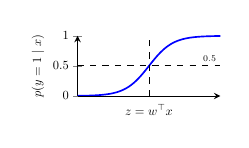
\begin{tikzpicture}[scale=0.75, every node/.style={scale=0.6}]
\begin{axis}[
  width=4cm, height=2.6cm,
  axis lines=left,
  xmin=-6, xmax=6,
  ymin=0, ymax=1,
  xtick=\empty, ytick={0,0.5,1},
  yticklabels={$0$,$0.5$,$1$},
  xlabel={$z=w^\top x$},
  ylabel={$p(y=1\mid x)$},
  domain=-6:6,
  samples=200,
]
% Sigmoid curve
\addplot[thick, blue] {1/(1+exp(-x))};

% 0.5 threshold line
\draw[dashed] (axis cs:-6,0.5) -- (axis cs:6,0.5);
\draw[dashed] (axis cs:0,0) -- (axis cs:0,1);

% Small label
\node[anchor=south east] at (axis cs:6,0.5) {\scriptsize $0.5$};
\end{axis}
\end{tikzpicture}

        \item \(\phi(z) = \dfrac{1}{1 + e^-z}\) (definition von funktion Z)
        \item \(p(y=1|x_i) = \phi(\beta_0 + x_i\beta_1)\) (Wahrscheinlichkeit klasse y)
        \item \(p(y=0|x_i) = 1- \phi(\beta_0 + x_i\beta_1)\) (Wahrscheinlichkeit andere klasse als y)
        \item \(\hat{y} = arg \; max  \;  p(y = k | x_1)\) (maximum davon \(\rightarrow\) predicted klasse)
        \item Kann auch konfiguriert werden dass es schon ab eg. 20\% Klasse 1 predicted
    \end{itemize}
    \item \textbf{Metrik}
    \begin{itemize}
        \item Was sind für Fälle möglich pro Datenpunkt
        \item Accuracy (nicht gut für inbalanced)
        \item F1-Score (gut bei inbalanced)
        \item Confusion Matrix keine Metrik und nicht immer aussagekräftig
    \end{itemize}
    \item \textbf{Kostenfunktion}
    \begin{itemize}
        \item Maximum Likelihood
        \item Sigmoid \(\phi\): Beweiss für eine Klasse
        \item Softmax: Beweiss für mehrere Klassen
    \end{itemize}
    \item \textbf{Optimierung}
    \begin{itemize}
        \item Gradient Descent auf Max Likelihood anwenden
    \end{itemize}
  \end{itemize}

\vspace{0.4em}
\hrule
\vspace{0.7em}

{\scriptsize{K-Nearest Neighbours}} Supervised Classification
  \begin{itemize}
    \item \textbf{Input}: Kontinuierlich or Diskret / \textbf{Output}: Diskret (category)
    \item \textbf{Beschreibung}
    \begin{itemize}
        \item Wir lernen keine \(\beta\)
        \item Wir suchen die nächsten k Punkte im train set (basierend auf mehrzahl)
        \item k ist Hyperparameter
        \item Keine Optimierung, keine Kostenfunktion
    \end{itemize}
    \item \textbf{Data Specification}
    \begin{itemize}
        \item Vorgabe: Was ist ziel variabel, was sind features?
        \item Encode Kategorsiche Features
        \item Standardisie Nummerische Features
    \end{itemize}
    \item \textbf{Model}
    \begin{itemize}
        \item \textbf{Curse of Dimensionality}
        \begin{itemize}
            \item Nicht gut bei vielen Features
            \item im hoch dimensionalen raum bedeutet distanz nicht viel
        \end{itemize}
    \end{itemize}
  \end{itemize}

\vspace{0.4em}
\hrule
\vspace{0.7em}

{\scriptsize{Support Vector Machine}} Supervised Classification
\vspace{-0.7em}

\begin{multicols}{2}

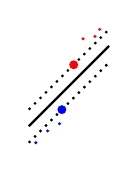
\begin{tikzpicture}[scale=0.3]
  % --- Decision boundary and margins (parallel) ---
  % Decision boundary: y = x
  \draw[thick] (-1.7,-1.7) -- (1.7,1.7);

  % Margins: y = x + 0.7 and y = x - 0.7
  \draw[dotted, thick] (-1.7,-1.0) -- (1.7,2.4);
  \draw[dotted, thick] (-1.7,-2.4) -- (1.7,1.0);

  % --- Class 1 (blue) points (below lower margin) ---
  \fill[blue] (-1.4,-2.4) circle (2pt);
  \fill[blue] (-0.9,-1.9) circle (2pt);
  \fill[blue] (-0.4,-1.6) circle (2pt);

  % Support vector (blue) on lower margin: y = x - 0.7
  % example: x=-0.3 -> y=-1.0
  \fill[blue] (-0.3,-1.0) circle (2pt);
  \draw[blue, very thick] (-0.3,-1.0) circle (3.2pt);

  % --- Class 2 (red) points (above upper margin) ---
  \fill[red] (0.6,2.0) circle (2pt);
  \fill[red] (1.1,2.1) circle (2pt);
  \fill[red] (1.3,2.4) circle (2pt);

  % Support vector (red) on upper margin: y = x + 0.7
  % example: x=0.2 -> y=0.9
  \fill[red] (0.2,0.9) circle (2pt);
  \draw[red, very thick] (0.2,0.9) circle (3.2pt);

\end{tikzpicture}


Support vectors: fat points

Decision boundary: fat line (hard margin, best division)

Soft margin: Decision boundary that allows for some flexibility

\end{multicols}
\vspace{-1.7em}

  \begin{itemize}
    \item \textbf{Input}: Kontinuierlich or Diskret / \textbf{Output}: Diskret (category)
    \item \textbf{Beschreibung}
    \begin{itemize}
        \item Support Vektoren: Punkte die die Decision Boundary Entscheiden (kleine Anzahl)
        \item Hoch dimensional möglich
        \item Keine wahrscheinlichkeit bei mehreren klassen ist nicht möglich
        \item es ist möglich mehrere modelle zu trainieren kann aber schnell gross werden bei mehreren klassen
        \item logistische regression ist meistens besser
    \end{itemize}
    \item \textbf{Data Specification}
    \begin{itemize}
        \item Vorgegebene kategorische Zielvariabel
        \item Feature selection
        \item Encode Kategorische
        \item Standardisie Nummerische
    \end{itemize}
    \item \textbf{Model}
    \begin{itemize}
        \item Heaviside Step Function 
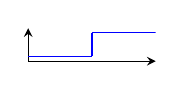
\begin{tikzpicture}
\begin{axis}[
  width=3.2cm, height=2.0cm,
  axis lines=left,
  xmin=-3, xmax=3,
  ymin=-0.2, ymax=1.2,
  xtick=\empty, ytick=\empty,
]
\addplot[blue] coordinates {(-3,0) (0,0)};
\addplot[blue] coordinates {(0,0) (0,1)};
\addplot[blue] coordinates {(0,1) (3,1)};
\end{axis}
\end{tikzpicture}
        
        \item Binäre Entscheidung, keine Wahrscheinlichkeit, kein softmax möglich
        \item One-vs-one Verfahren, sprich ein modell pro Klassen-Paar 1 vs. 2 / 2 vs. 3 / 3 vs. 1, precit klasse mit meisten votes
        \item Decision Boundary ist linie mit maximalen Abstand zum nächsten Punkt der anderen Klasse
        \item Geometrische Annahmen
    \end{itemize}
    \item \textbf{Kostenfunktion}
    \begin{itemize}
        \item wenn C sehr gross ist dann wird cheating minimiert (stärker bestraft) und umgekehrt, das sind hyper-parameter 
        \item wenn ich C kleiner mache kann die margin grösser werden und mehr datenpunkte verletzten die margin
        \item Cheating darf nicht negativ sein, man darf nur in die selbe richtung cheaten nicht bei einer positiv und bei einer anderen negativ
        \item Es gibt immer eine lösung, aber es kann sein, dass das cheating relativ gross sein muss um eine lösung zu haben
    \end{itemize}
    \item \textbf{Optimierung}
    \begin{itemize}
        \item Hard margin (solver gibt \(\beta\) zurück)
        \item Maximise \(M\), subject to \(||\beta|| = 1\), subject to \(\beta x^{(i)} \ge M\), subject to \(-(\beta x^{(i)}) \ge M\)
        \item Soft margin (bei hard margin gäbe es daten bei denen es keine lösung gibt), robust for outliers, applicably to non-linear data, but need for parameter tuning, and may overfit
        \item bei jeder variabel darf die margin ein wenig abweichen um einen "cheat" wert (zeta) das ist ein hyperparameter
        \item aber wir müssen sagen, dass in der summe möglichst wenig verletzt werden
    \end{itemize}
  \end{itemize}

\vspace{0.4em}
\hrule
\vspace{0.7em}

{\scriptsize{Decision Trees}} Supervised Classification

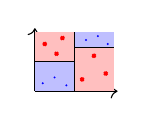
\begin{tikzpicture}[scale=0.25]
  % Axes
  \draw[->] (0,0) -- (4.2,0);
  \draw[->] (0,0) -- (0,3.2);

  % --- Regions (2 classes) ---
  % Blue regions
  \fill[blue!25] (0,0) rectangle (2,1.5);
  \fill[blue!25] (2,2.2) rectangle (4,3);

  % Red regions
  \fill[red!25]  (2,0) rectangle (4,2.2);
  \fill[red!25]  (0,1.5) rectangle (2,3);

  % --- 4 Cuts (split lines) ---
  % vertical cuts (2)
  \draw (2,0) -- (2,3);

  % horizontal cuts (2)
  \draw (0,1.5) -- (2,1.5);
  \draw (2,2.2) -- (4,2.2);

% --- Data points ---
  % Blue points (class 1)
  \foreach \p in {(0.4,0.4),(1.0,0.7),(1.6,0.3),(2.6,2.6),(3.2,2.8),(3.7,2.4)}
    \fill[blue] \p circle (1.6pt);

  % Red points (class 2)
  \foreach \p in {(2.4,0.6),(3.6,0.9),(3.0,1.8),(0.5,2.4),(1.4,2.7),(1.1,1.9)}
    \draw[red, thick] \p ++(-0.08,-0.08) -- ++(0.16,0.16)
                     \p ++(-0.08, 0.08) -- ++(0.16,-0.16);

\end{tikzpicture}


  \begin{itemize}
    \item \textbf{Beschreibung}
    \begin{itemize}
        \item Kann keine extrapolation machen für Daten ausserhalb der Trainingsdaten (können nur interpolation auch wenn es eine sinnvolle extrapolation geben würde)
        \item Ziel: Feature-space in regionen aufteilen
        \item Kann nicht lineare zusammenhänge lernen
        \item Robst bei vielen Features, weil unwichtige selten/nicht für splits verwendet werden
        \item Wird of in einem ensemble verwendet und nicht alleine
        \item Gut interpretierbar
    \end{itemize}
    \item \textbf{Data Specification}
    \begin{itemize}
        \item Vorgegebene kategorische Zielvariabel
        \item Feature selection
        \item Encode Kategorische
        \item Standardisie Nummerische features wenn nicht gleiche
    \end{itemize}
    \item \textbf{Model}
    \begin{itemize}
        \item Abbruch bedingung setzten als hyper parameter, eg. maximale Tree Tiefe
        \item wenn keine abbruch bedingung dann soweit bis alles sauber ist
        \item Wahrscheinlichkeit für klasse \(k\) for Region \(R_m\) gibt es zurück
        \item Kann extrem overfitted sein
        \item Möglich nachträglich baum zu reinigen
        \item \(p(y=k|R_m) = \frac{1}{N_m} \sum_{x^{(i) \in R_m}} I(y^{(i)} = k\)
        \item Klasse mit höchster Wahrscheinlichkeit vorhersagen für Region \(R_m\)
        \item \(\hat{y}_{R_m} = arg\;max\;p(y = k|R_m)\) 
    \end{itemize}
    \item \textbf{Kostenfunktion}
    \begin{itemize}
        \item Impurity (Verunreinigung) der Regionen messen
        \item Welche funktion genommen wird ist hyperparameter
        \item Wir können auch unterschiedliche Bäume vergleichen
    \end{itemize}
    \item \textbf{Optimierung}
    \begin{itemize}
        \item Theorie: es gibt einen perfekten Baum für testdaten. Aber rechenintensiv und overfittet
        \item Praxis: guter Tree mit einem Greedy Altgorithmus finden. Making a locally optimal decision, in the hope of reaching a global optimum
        \item robust bei vielen features.
        \item Greedy: Finde besten Split für aktuelle Region \(R\) zum unterteilen in \(R_1\) und \(R_2\) nach \(M\), Bestes Feature (f) mit bestem Threshold (t)
        \item Wiederholt angewendet auf \(R_1\) und / oder \(R_2\) je nach Abbruchbedingung.
    \end{itemize}
    \item \textbf{Random Forest}
    \begin{itemize}
        \item Trainiere viele Decision Trees auf zufällige Tiele der Daten
        \item Finale prediction ist durchschnitt der trainierten decision trees
        \item Enseble methode genannt Bagging
    \end{itemize}
  \end{itemize}

\vspace{0.4em}
\hrule
\vspace{0.7em}

{\scriptsize{Clustering}} Unsupervised Classification
  \begin{itemize}
    \item \textbf{Beschreibung}
    \begin{itemize}
        \item Zusammenhänge in Datenwolken finden
    \end{itemize}
    \item \textbf{Model}
    \begin{itemize}
        \item eg. k-means algorithmus
        \item Anzahl k festlegen
        \item sucht minimale distanz
    \end{itemize}
  \end{itemize}

\vspace{0.4em}
\hrule
\vspace{0.7em}

{\scriptsize{Principal Component Analysis}} Unsupervised Dimensionality Reduction
  \begin{itemize}
    \item \textbf{Beschreibung}
    \begin{itemize}
        \item 1. Wir suchen Principal Components (Hauptkomponenten) des Datensatztes. Das ist die achse die am meisten streuung ausdrückt. 
        \item 2. Wir projezieren die Daten darauf
        \item 3. Wir suchen eine neue achse die rechtwiklig darauf liegt, etc.
        \item Die Hauptkomponenten werden zu unserem neuen Koordinaten system (features). Die achsen haben für uns intuitiv keine bedeutung mehr
        \item Im PC-Space machen wir dann "Feature Selection", sprich wir behalten nur die wichtigsten Hauptkomponenten (neuen "Features")
        \item weniger informationsverlust aber etwas geht verloren
        \item Wann?: performanz optimierung (speed-up, less memory)
        \item Wann nicht?: overfitting, da ist regularisierung meist bessere wahl
    \end{itemize}
    \item \textbf{Data Specification}
    \begin{itemize}
        \item Welche features gibt es, eg. Pixel
        \item keine zielvariabel
        \item kategorische encoded
        \item nummerische standardisiert
    \end{itemize}
    \item \textbf{Annahme}
    \begin{itemize}
        \item gesuchtes Manifold ist linear
        \item kann nichts anderes, aber vieles ist nicht-linear
    \end{itemize}
    \item \textbf{Model}
    \begin{itemize}
        \item encoder: \(L = xW\) lineare Abbildung, Matrix W
        \item decoder: \(\hat{x} = xWW^T\) rekonstruktion x (automatisch dabei)
        \item Anzahl Dimension? Wie viel streeung verlieren wir wenn wir auf x komponenten gehen? \\
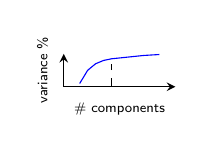
\begin{tikzpicture}
\begin{axis}[
  width=3cm, height=2cm,
  axis lines=left,
  xmin=0, xmax=7,
  ymin=0, ymax=1,
  xtick=\empty, ytick=\empty,
  xlabel={\tiny \# components},
  ylabel={\tiny variance \%},
]
% Reverse elbow (fast increase then plateau)
\addplot[blue] coordinates {
  (1,0.10) (1.5,0.5) (2,0.7) (2.5,0.8) (3,0.85) (4,0.90) (5,0.95) (6,0.98)
};
% Optional "elbow" marker line (at k=3)
\draw[dashed] (axis cs:3,0) -- (axis cs:3,0.70);
\end{axis}
\end{tikzpicture}

    \end{itemize}
    \item \textbf{Kostenfunktion}
    \begin{itemize}
        \item L2-Distanz der Rekonstruktion \(\hat{X}\) (Encoder \(W\) / Decoder \(W^T\) sind Matrix)
        \item \(J(W) = || X - \hat{X} ||_2 = || X - XWW^T ||_2\)
    \end{itemize}
    \item \textbf{Optimierung}
    \begin{itemize}
        \item "Einfache" Lineare Algebra, nutzt singular value decomposition
        \item Wir nehmen die minimale Matrix \(W\)
    \end{itemize}
  \end{itemize}

\vspace{0.4em}
\hrule
\vspace{0.7em}

{\scriptsize{Non-Negative Matrix Factorisation}} Unsupervised Dimensionality Reduction
  \begin{itemize}
    \item \textbf{Beschreibung}
    \begin{itemize}
        \item Input Matrix in zwei kleinere Faktorisieren, die wenn sie zusammen multipliziert werden die beste rekonstrutkion der anfangs matrix sind.
        \item Es liefert keinen Encoder (\(A / B\) wird nicht gespeichert, also nicht für pre-processing für Supervised Learning Task geeignet.
        \item wird jedes mal neu berechnet
        \item Motivation: Addition von non-negativen Konzepten (hidden features) macht andere konzepte verständlicher
    \end{itemize}
    \item \textbf{Data Specification}
    \begin{itemize}
        \item Wleche features, eg. Pixel
        \item Anzahl \(k\) is als hyperparameter vorgegeben
        \item Nur positive werte, wert features \(\geq\) 0
        \item Features müssen einheitliche grössen haben
    \end{itemize}
    \item \textbf{Model}
    \begin{itemize}
        \item Ziel: \(X_{n\cdot m} \approx A_{n \cdot k} \cdot B_{k \cdot m}\)
        \item \(k \leq min(n, m)\)
        \item Ziel: Rekonstruierte Matrix ungefähr gleich hohe matrix A mal breite matrix B
        \item \(X\) Feature matrix \(\rightarrow\) Encoder \(\rightarrow\) \(A\) kleine Matrix \(\rightarrow\) Decoder (\(B\)) \(\rightarrow\) \(AB\)
    \end{itemize}
    \item \textbf{Metrik}
    \begin{itemize}
        \item 
    \end{itemize}
    \item \textbf{Kostenfunktion}
    \begin{itemize}
        \item Gleiche wie bei PCA
        \item \(J(A, B) = || X - \hat{X}||_2 = || X - AB ||_2\)
    \end{itemize}
    \item \textbf{Optimierung}
    \begin{enumerate}
        \item Initialisiere A, B mit zufälligen Werten
        \item Optimiere A nach Kostenfunktion, B bleibt fix (optimiere räpresentation gegeben Decoder B)
        \item Optimiere B nach Kostenfunktion, A bleibt fix (optimiere decoder gegeben repräsentation A)
        \item Wiederhole 2. und 3. bis nur noch wenig veränderung statt findet
        \item[-] Findet lokales minimum. Ganzen Algorithmus mehrmals wiederholen mit anderen initialwerten, anderes resultat
    \end{enumerate}
  \end{itemize}

\vspace{0.4em}
\hrule
\vspace{0.7em}

{\scriptsize{Fully Connected Neural Network}}
  \begin{itemize}
    \item FCNN = Multi Layer Perceptron = Neural Network
    \item \textbf{Beschreibung}
    \begin{itemize}
        \item Input Layer (dimension anzahl features) \(\rightarrow\) Hidden Layer  \(\rightarrow\)  ...  \(\rightarrow\) Output Layer (dimension anzahl resultate)
        \item Aktivierungsfunktion: Transformierung vom wert bevor er weitergegeben wird
    \end{itemize}
    \item \textbf{Data Specification}
    \begin{itemize}
        \item Was ist das Ziel
        \item Was ist die Kostenfunktion
        \item Feature selection
        \item Kategorische müssen encoded werden
        \item Nummerische standardisiert
    \end{itemize}
    \item \textbf{Model}
    \begin{itemize}
        \item \(\phi\) Aktivierungsfunktion macht das Modell nicht-linear, beliebteste ReLU
        \item eg. Logisitsche Regression als neurales netzwerk mit aktivierungsfunktion \(\phi\)
        \item \(\hat{y} = \phi(\beta_0 + \beta_1x_1 + ...)\)
        \item Mehrere Outputs möglich dann für das letzte layer ist die aktivierungsfunktion der soft-max
        \item Softmax: amplifies largest value so that it is closer to 1
    \end{itemize}
    \item \textbf{Kostenfunktion}: oben
    \item \textbf{Optimierung}
    \begin{itemize}
        \item Gradient Descent
        \item Stochastic Gradient Descent
        \begin{itemize}
            \item 1 sample \(\rightarrow\) richtung minimum
            \item update sehr schnell berechnet, oftmals in falsche richtung, sehr noisy
        \end{itemize}
        \item Min Batch Gradient Descent
        \begin{itemize}
            \item x samples richtung minimum
            \item update schnell, weniger noisy als stochastic
        \end{itemize}
    \end{itemize}
  \end{itemize}


\vspace{0.4em}
\hrule
\vspace{0.7em}

{\scriptsize{Auto Encoder}} Unsupervised Dimensionality Reduction

Reconstruction based Method

  \begin{itemize}
    \item \textbf{Beschreibung}
    \begin{itemize}
        \item lerne nicht-lineares Manifold im Feature-Space
      \item Nicht-lineare Dimensionality Reduction anhand von Daten lernen.
      \item Wir verwenden ein Neural Network und den Reconstruction Error als Kostenfunktion.
      \item Undercomplete Autoencoder:
        \begin{itemize}
          \item Bottleneck in der Architektur des Netzwerks.
          \item wichtige info verdichten, unwichtiges weglassen
          \item Input 300 Pixel, Latent space 20 fetaures, reconstructed input space 300 pixel
        \end{itemize}
      \item Overcomplete Autoencoder:
        \begin{itemize}
          \item Kein Bottleneck, aber Regularization.
        \end{itemize}
        \item Aktivierungsfunktion muss nicht linear sein
        \item genaue Architektur (no. hidden layers, nodes, etc) ist hyperparameter
    \end{itemize}
    \item \textbf{Data Specification}
    \begin{itemize}
        \item features? (eg. pixel)
        \item kategorische encoden
        \item nummerische standardisieren
    \end{itemize}
    \item \textbf{Model}
    \begin{itemize}
        \item 
    \end{itemize}
    \item \textbf{Metrik}
    \begin{itemize}
        \item 
    \end{itemize}
    \item \textbf{Kostenfunktion}
    \begin{itemize}
        \item Rekonstruktionsfehler: \(J(\beta) = ||X-\hat{X}||_2\)
        \item Andere auch möglich z.b. L1 Distanz
    \end{itemize}
    \item \textbf{Optimierung}
    \begin{itemize}
        \item Gradient Descent
    \end{itemize}
    \item \textbf{Limits}
    \begin{itemize}
        \item Reconstruction Error, nicht optimal für z.b. Bilder
        \item Gelerntes beinhaltet viel pixel-perfekt statt semantische informationen
    \end{itemize}
    \item Wenn Encoder \& Decoder Linear sind (lineare aktivierungsfunktion), dann lernt der Auto Encoder den gleichen Latent Space wie PCA
  \end{itemize}

  
\end{multicols}

\hrule
\vspace{0.4em}
\hrule


\begin{multicols}{5}

\scriptsize

{\footnotesize{\textbf{Optimisation}}}

\begin{itemize}
    \item Optimisation wird von der Kostenfunktion geleitet.
    \item Mechanismus wie wir die \(\beta\) (lernbare parameter) eines Modells für eine \textbf{Kostenfunktion} aus \textbf{Daten lernen}.
    \item unterschiedliche mit anderen eigenschaften / präferenzen  \(\rightarrow\) Performanz (Zeit), Genearlisierung (Qualität)
    \item Wenn visualisierung von optimalen \(\beta\) eine Schüssel \(\rightarrow\) Convex Kostenfunktion
\end{itemize}


\vspace{0.4em}
{\scriptsize{\textbf{Optimisation Algorithm}}}
      \begin{itemize}
      \item {\textbf{Analytische Methode}}
      \begin{itemize}
          \item nicht iterativ (löst die Normalgleichung)
          \item besser bei wenigen features
          \item Matrix muss invertierbar sein
      \end{itemize}
      \item \textbf{Gradient Descent}
      \begin{itemize}
          \item Iterativ, Start zufällige \(\beta\)
          \item Ableitung der Kostenfunktion
          \item mit jedem Schritt in die bessere richtung, bis zum minimum
          \item gut für viele Daten und \(\beta\)
      \end{itemize}
    \end{itemize}


\vspace{0.4em}
\hrule
\vspace{0.7em}


{\scriptsize{\textbf{Metrik}: Regression}}
\begin{itemize}
  \item \textbf{Mean Absolute Error (MAE)}
  \begin{itemize}
      \item \(\frac{1}{n}\sum_{i=1}^{n} \left| y_i - \hat{y}_i \right|\)
      \item robust gegen ausreisser
      \item Fehler $>$ 1 start bestraft
      \item Fehler $<$ 1 schwächer bestraft
  \end{itemize}
\item \textbf{Mean Square Error (MSE)}
  \begin{itemize}
      \item \(\frac{1}{n}\sum_{i=1}^{n} \left( y_i - \hat{y}_i \right)^2\)
      \item beieinflusst von Ausreisser
      \item bestraft grosse Fehler stark
  \end{itemize}
\end{itemize}

\vspace{0.4em}
{\scriptsize{\textbf{Metrik}: Klassifikation}}

\begin{itemize}
    \item True Positive \(\rightarrow\) TP / True Negative \(\rightarrow\) TN, etc
    \item \textbf{Accuracy}
      \begin{itemize}
            \item \(\dfrac{TP + TN}{TP + TN + FP + FN}\)
            \item irreführend bei inbalanced klassen
            \item 99 A und 1 B, wenn immer A dann gute accuracy auch wenn Modell dumm
      \end{itemize}
    \item \textbf{Precision}
        \begin{itemize}
            \item \(\dfrac{TP}{TP + FN}\)
        \end{itemize}
    \item \textbf{Recall}
    \begin{itemize}
        \item \(\dfrac{TP}{TP + FN}\)
  \end{itemize}
  \item \textbf{F1-Score}
    \begin{itemize}
        \item \(F_1 = 2 \cdot \dfrac{Precision \cdot Recall}{Precision + Recall}\)
        \item gut bei inbalanced klassen
    \end{itemize}
\end{itemize}


TODO: Bestimmtheitsmass \(R^2\)


\vspace{0.4em}
\hrule
\vspace{0.7em}

{\footnotesize{\textbf{Kostenfunktion}}}

\begin{itemize}
    \item Guides Optimisation
    \item Minimise errors, improve model accuracy, used during training
\end{itemize}


{\scriptsize{\textbf{Maximum Likelihood}} Klassification}
\begin{itemize} 
    \item TODO: furuther investigation
    \item wahrscheinlichkeit für einen datenpunkt * wahrscheinlichkeit aller anderen
    \item Wert möglichst nahe 1 \(\rightarrow\) Wahrscheinlichkeit für eine Klasse
    \item Resultat: Wie wahrschienlich sind die labels die ich habe und unserem Modell
    \item Je mehr Datenpunkte desto näher bei 0, aber immernoch vergleichbar
    \item we wish to maximize the conditional probability of observing the data (X) given a specific probability distribution and its parameters
    \item \( p(\overrightarrow{y} | X ) = \prod \phi(x^i\beta) \cdot \prod{1-\phi(x^i\beta)}\) \\
    probability feature \(x_i \rightarrow\) +ve sample * -ve Sample 
\end{itemize}




\vspace{0.4em}
\hrule
\vspace{0.7em}

{\footnotesize{\textbf{Feature Preprocessing}}}

{\scriptsize{\textbf{Encoding}}}

\begin{itemize}
    \item Information in anderer Maschienen freundlichen Art darzustellen.
    \item oft notwendig für text
    \item mit oder ohne Informationsverlust

\item \textbf{Kategorisch}
\begin{itemize}
    \item \textbf{Ordinal}
    \begin{itemize}
        \item mapping von kategorie mit aufsteigender Zahl 0-n
        \item 1 Feature \(\rightarrow\) 1 Feature
        \item hat eine Ordnung, grösse der Zahl hat einen Einfluss!
        \item nicht gut wenn es keine Ordnung hat oder Abstände nicht regelmässig
        \item eg. Kleidergrössen xs-xl (0-4) könnte passen weil es hat eine inherente bedeutung
    \end{itemize}
    \item \textbf{One-Hot}
    \begin{itemize}
        \item n-Einzigartige Eigenschaften \(\rightarrow\) n-Dimensionalen Vektoren
        \item 1 Feature \(\rightarrow\) n Feature
        \item Vektor, 0/1, 1 eintrag wo es in der reihenfolge stimmt, sonst 0
    \end{itemize}
    \item Meistens one-hot da ordnung nichts bedeutet
    \item Domänenwissen kann einfliessen zum eg. neue Kategorien zu bilden
\end{itemize}

\item Meistens One-Hot weil Dinge keine Ordnung haben
\item Möglich mit Domänen-Wissen eigene Encoding machen (eg. Kategorien zusammenfassen)
\end{itemize}

\vspace{0.4em}
{\scriptsize{\textbf{Feature Selection}}}

\begin{itemize}
    \item Auswahl von Features die relevant sind, einfacher für das Modell
    \item overfittet nicht auf features die nicht relevant sind
    \item Ansätze
    \begin{itemize}
        \item Manuell mit Domänenwissen (schwierig)
        \item Automatisch Ausschliessen von features die nichts mit der Zielvariabel zu tun haben
    \end{itemize}
\end{itemize}

\vspace{0.4em}
{\scriptsize{\textbf{Standardise}}}
\begin{itemize}
    \item Schiebt alles um 0 Punkt
    \item Entfernt Einheiten, separat pro Feature, erhält Verhältnisse
    \item notwendiger Schritt sodass Modelle richtig funktionieren
    \item Wann?: Parameter müssen vergleichbar sein
    \item Wann?: Distanzen im input space spielen eine Rolle, ansonsten haben grosse Werte einen einfluss
    \item Meist \texttt{StandardScaler} = \(\dfrac{Wert - Durchschnitt}{Standardabweichung}\)
\end{itemize}

\vspace{0.4em}
{\scriptsize{\textbf{Dimensionality Reduction}}}

\begin{itemize}
    \item Manifold-Annahme: Hochdimensionale Daten liegen auf einem tiefer-dimensionalen Manifold
    \item wir möchten möglichst viel streuung erhalten
    \item Eg. 3072 Pixels / Features. Dimensionsreduktion: Finde x nummer neue features (eg. 200) die die Daten präzieser Beschreiben können. Viele Pixel sind nicht zwingen aussagekräftig.
    \item Input Space (3072 Pixels / features) \(\rightarrow\) Latent Space (200 features)
    \item Input Space: 1'000 1-hot encoded words \(\rightarrow\) Latent Space (300 features)
    \item Wird gelern auf einem ganzen Datensatz (nicht einen Teil)
    \item Die zugrundeliegende Struktur im Datensatz wird gelernt
    \item Die gelernte Reduktion kann dann auf neue Daten und die daten selbst angewandt werden
    \item Einsatzgebiet: Feature Preprocessing, Interpretation der Daten (Visualisierung / Faktor-Analyse), Wörter original synonyme gleiche distanz, encoded wird grouppiert
    \item Bei zu vielen features kann das Gewicht am falschen ort gesetzt werden
    \item performanz optimierung
    \item zu wenige Daten dann overfitting, aber bessere (aussagekräftigere features) \(\rightarrow\) besseres lern-ausgangslage
    \item Feature Selection as Dim. Reduction \(\rightarrow\) wir lassen info weg, problem grosser informationsverlust
    \item Idee: Wir reduzieren die Anzahl features indem wir weniger neue features erstellen (weniger informationsverlust)
\end{itemize}

\vspace{0.4em}
\hrule
\vspace{0.7em}

{\footnotesize{\textbf{Feature Engineering}}}

{\scriptsize{\textbf{Explizit}}}

\begin{itemize}
    \item Bestehende features \(\rightarrow\) neue features
    \item expertenwissen, nimmt einen Teil des Learning Ab \(\rightarrow\) gibt wissen vor.
    \item {\textbf{Polynomielle Regression}} (Standard)
    \begin{itemize}
        \item Input Space: \texttt{x}
        \item Feature Engineering \(\rightarrow\) Feature Space: \texttt{x}, \texttt{$x^2$}
        \item Modell \(\rightarrow\) Output Space: \texttt{y}
        \item E.g. Volumen von Fisch berechnen, so kann regression Polynome haben
    \end{itemize}
    \item Sind besser auf trainings daten, nicht immer besser auf test daten
\end{itemize}

\vspace{0.4em}
{\scriptsize{\textbf{Kernel Trick}}}

\begin{itemize}
    \item Normal: wir loopen über anzahl Features \(\rightarrow\) implizites feature engineering
    \item Kernel Trick: wir loopen über anzahl daten \(\rightarrow\) kernel macht modelle nicht linear
    \item Schlecht bei vielen Daten (aber z.b. SVM hat wenige support vekotren, sprich wenig daten)
    \item Transformation into higher dimensions where it can be separated linearly is good, but Problem: high dimensions are expensive
    \item Es macht zwischen input and model implizites feature engineering un löst die kosten der höheren dimenensionen.
    \item We compute result without having to explicitly compute the intermediary higher dimension. Through Representer Theorem
\end{itemize}

\vspace{0.4em}
\hrule
\vspace{0.7em}


{\footnotesize{\textbf{Modell Komplexität}}}

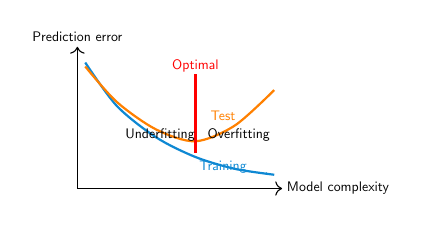
\begin{tikzpicture}[scale=0.5, every node/.style={scale=0.5}]
  % Axes
  \draw[->] (0,0) -- (5.2,0) node[right]{Model complexity};
  \draw[->] (0,0) -- (0,3.6) node[above]{Prediction error};

  % Training curve (decreasing)
  \draw[thick, cyan!70!blue]
    plot[smooth] coordinates {(0.2,3.2) (1,2.1) (2,1.3) (3,0.8) (4,0.5) (5,0.35)};
  \node[circle, fill=cyan!70!blue, inner sep=0.7pt] at (4.8,0.38) {};
  \node[cyan!70!blue] at (3.7,0.55) {Training};

  % Test curve (U-shaped)
  \draw[thick, orange]
    plot[smooth] coordinates {(0.2,3.1) (1,2.2) (2,1.5) (3,1.2) (4,1.6) (5,2.5)};
  \node[orange] at (3.7,1.85) {Test};

  % Optimal vertical line
  \draw[red, thick] (3,2.9) -- (3,0.9);
  \node[red] at (3,3.1) {Optimal};

  % Under/Overfitting labels
  \node at (2.1,1.35) {Underfitting};
  \node at (4.1,1.35) {Overfitting};
\end{tikzpicture}


{\scriptsize{\textbf{Overfitting vs. Underfitting}}}

\begin{itemize}
    \item \textbf{Overfitting}: super training, schelcht test
    \item \textbf{Underfitting}: schlecht training schlecht test
    \item Je komplexer das Modell desto höher die Gefahr für overfitting
\end{itemize}

\vspace{0.4em}
{\scriptsize{\textbf{Cross Validation}}}

\begin{itemize}
    \item vergleich von verschiedenen ML Modell-Arten
    \item Gefahr: falsches Modell, nur durch Zufall gut, mehr validierungsdaten, desto unwahrscheinlicher
    \item 2 Strategien
    \begin{itemize}
        \item Hold out Corss validation: Train, Val, Test (no peeking)
        \item k-Fold mehr validierungsdaten herbeizaubern
    \end{itemize}
    \item K-Fold Cross Validation
    \begin{itemize}
        \item Alle Daten sind im validierungsset
        \item Iterativ üver alle Segmente gehen
        \item Mehr rechenzeit, aber weil wenig daten nicht ein problem
    \end{itemize}
\end{itemize}

\vspace{0.4em}
{\scriptsize{\textbf{Regularisation}}}
\begin{itemize}
    \item Annahme: Grosse \(\beta\) zeichen für overfitting, sollten nahe 0 sein, Modell wird einfacher
    \item Daten müssen Standard Skaliert werden
    \item Regularisierungsstärke \(\lambda \rightarrow\) ist Hyperparameter
    \item Grosses \(\lambda \rightarrow\) stark konfiguriert \(\beta\) näher bei 0
    \item {\textbf{L1 Lasso}}: Absolut \(|\beta|\)
    \begin{itemize}
        \item Grosse \(|\beta|\) werden bestraft
        \item Gut für automatische Feature-Selection (unwichtiges \(|\beta|\) verschwindet)
        \item \(J_{\text{Reg}}(\beta) = J(\beta) + \lambda \sum_{j=1}^{p} |\beta_j|\)
    \end{itemize}
        \item {\textbf{L2 Ridge}}: Quardrat \(\beta^2\)
    \begin{itemize}
        \item \(|\beta|\) nahe 0 sonst bestraft
        \item Zahlen unter 1 weniger bestraft als bei L1
        \item Alle \(|\beta|\) klein, ausgewogen in vergleich zu L1
        \item \(J_{\text{Reg}}(\beta) = J(\beta) + \lambda \sum_{j=1}^{p} \beta^2_j\)
    \end{itemize}
\end{itemize}

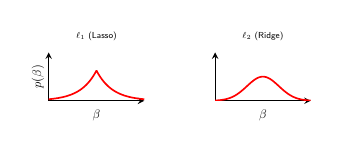
\begin{tikzpicture}[scale=0.75, every node/.style={scale=0.6}]

\begin{groupplot}[
  group style={group size=2 by 1, horizontal sep=1.2cm},
  width=3.2cm, height=2.4cm,
  axis lines=left,
  xtick=\empty, ytick=\empty,
  xmin=-3, xmax=3,
  ymin=0, ymax=0.8,
  domain=-3:3,
  samples=200,
  xlabel={$\beta$},
  ylabel style={at={(axis description cs:0,0.5)},anchor=south},
]

% ---------- L1 (Laplace) ----------
\nextgroupplot[
  title={\scriptsize $\ell_1$ (Lasso)},
  ylabel={$p(\beta)$}
]
\addplot[red, thick] {0.5*exp(-abs(x))};  % Laplace(0,1)

% ---------- L2 (Gaussian) ----------
\nextgroupplot[
  title={\scriptsize $\ell_2$ (Ridge)}
]
\addplot[red, thick] {1/sqrt(2*pi)*exp(-x^2/2)}; % Normal(0,1)

\end{groupplot}
\end{tikzpicture}


\vspace{0.4em}
\hrule
\vspace{0.7em}


{\footnotesize{\textbf{Model Selection}}}

{\scriptsize{\textbf{Hyper Parameter}}}
\begin{itemize}
    \item Werden nicht gelernt \(\rightarrow\) konfiguriert das Modell
    \item Z.B. Regularisierungsstärke \(\lambda\), Anzahl Bäume (Random Forest), Anzahl Cluster (k-means), DL Netzwerk Architektur
    \item Wie wählen?
    \begin{itemize}
        \item Manuell: Erfahrung \& Theorie  \(\rightarrow\) schwierig
        \item Suchen: Ausprobieren und auf ungesehen Daten merken  \(\rightarrow\) Rechenintensiv
        \begin{itemize}
            \item \textbf{Grid Search:} Liste von Werten, ausprobieren, nicht gut bei vielen hyper Parameter wegen kombination
            \item \textbf{Randomised Search:} Zufällige Zahlen innerhalb eines vorgegebenen Bereiches
        \end{itemize}
    \end{itemize}
\end{itemize}

\vspace{0.4em}
\hrule
\vspace{0.7em}


{\footnotesize{\textbf{Deep Learning}}}

\begin{itemize}
    \item Deep Learning = ML mit Neuralen netzen als Modell
    \item Vorher: viele Annahmen + Wissen vorprogrammiert, Modell helfen
    \item trainiert auf manuelle räpresentation d.h. features und dimensionality reduction. Manuelle räpresentation für Bilder/Text schwierig
    \item Motivation DL: räpresentation automatisch aus Daten lernen
    \item kann supervised oder unsupervised sein
    \item viele Daten \& Rechenzeit
    \item Meist beste Wahl für unstrukturierte Daten (Bilder/Text) die viele features haben die alleine nicht aussagekräftig sind.
    \item Strukturierte Daten meist nicht die beste wahl
    \item \textbf{Framework für Modelle}
    \begin{itemize}
        \item Architektur NN ist problemspezifisch, und unterschiedlich Kombinierbar
        \item müssen empirisch evaluiert werden
        \item abwegung von black-box vs. komplexe probleme lösbar
      \item Modellkomplexität ist einfach anpassbar
        \begin{itemize}
          \item Mehr Hidden Layers $\rightarrow$ mehr lernbare Parameter.
          \item Weniger Hidden Layers $\rightarrow$ weniger lernbare Parameter.
          \item In einem Layer mehr Nodes $\rightarrow$ mehr lernbare Parameter.
          \item In einem Layer weniger Nodes $\rightarrow$ weniger lernbare Parameter.
        \end{itemize}
      \item Kostenfunktion
        \begin{itemize}
          \item Die Kostenfunktion muss ableitbar sein.
          \item Sie kann problemspezifisch gewählt werden.
        \end{itemize}
        \item Hidden Layer
        \begin{itemize}
            \item Zwischenergebnisse, kann als gelerntes feature engineering betrachtet werden
            \item feature engineering \(\rightarrow\) mehr aus weniger
            \item dimensionality reduction \(\rightarrow\) weniger aus mehr
        \end{itemize}
        \item Optimierung
        \begin{itemize}
            \item Gradient Descent mit Lokalem minmum, Unterschiedliche Lösungen möglich basierend startpunkt
        \end{itemize}
      \item Viele weitere Möglichkeiten (Deep Learning)
        \begin{itemize}
          \item Wir können die Architektur (Verbindungen) des Netzwerks anders gestalten,
                entsprechend dem zugrunde liegenden Problem.
          \item Beispiele: CNN und RNN.
        \end{itemize}
    \end{itemize}
\end{itemize}

{\scriptsize{\textbf{Beispiel}}}

\begin{itemize}
    \item \textbf{Convoluted Neural Network (CNN)}
    \begin{itemize}
        \item Annahme: Nachbarschaft von einem input (eg. Pixel) hat einen Einfluss and die anderen Pixel
        \item Wir verändern die verkabelung im netzwerk um den input besser zu berücksichtigen
        \item Input bleibt gleich gross
        \item wenn die nachbarschaft egal ist, dann ist es nicht die richtige wahl
    \end{itemize}
    \item \textbf{Contrastive Learning}
    \begin{itemize}
        \item eg. Gesichteserkennung
        \item kennt person, neue person muss maximale distanz von einander haben
        \item lernt wichtige aspekte im gesicht und unwichtiges (brille, haare) ignorieren
        \item One-Shot Learning, lernt neue Person (klasse) mit nur einem Bild
    \end{itemize}
    \item Zero-Shot Learning
    \begin{itemize}
        \item kann was machen mit nur 1 input
        \item eg. gemeinsamer laten space für Bilder und Text
        \item "an image of a dog" und kann damit einen output generieren
    \end{itemize}
    \item \textbf{Skip Connections}
    \begin{itemize}
        \item kreative Architektur
        \item viele Layers schwierig zu trainieren
        \item überspringt gewisse layers, parallel trainiert, \(\beta\) am schluss summiert
        \item Voraussetzung identische Dimensionen
    \end{itemize}
\end{itemize}


\vspace{0.4em}
\hrule
\vspace{0.7em}


{\footnotesize{\textbf{In-Context Learning}}}

\begin{itemize}
    \item auch prompting
    \item keine veränderung von \(\beta\)
    \item neues ist nur kontext
    \item Prompt Engineering: Prompt dem Modell anpassen damit es besser funktioniert
    \item \textbf{Zero-Shot}
    \begin{itemize}
        \item vorgabe\(\rightarrow\) task description (eg. translate)
        \item vorgegeben in natural language
        \item + user input
    \end{itemize}
    \item \textbf{Few/One-Shot}
    \begin{itemize}
        \item vorgabe\(\rightarrow\) task description + example
        \item + user input
    \end{itemize}
    \item Learning weil durch context (system promtps und beispiele) können wir das resultat verbessern
    \item RAG and Agentic AI
    \item ICL / LLM Limits
    \begin{itemize}
      \item Hallucination: Faktisch falsche Informationen, oft klingen sie plausibel.
      \item Knowledge Cutoff: Wissensstand veraltet (Training).
      \item Prompt Sensitivity: Formulierung und Struktur des Prompts überraschend wichtig.
      \item Fehlendes Weltverständnis/Logik: Kein echtes Verständnis, keine Kausalität oder robustes logisches Schlussfolgern.
      \item Hohe Kosten: Rechenressourcen und Energie.
      \item Verbesserung schwierig: Oft schneller Prototyp, aber der Weg zum Produkt ist nicht immer einfach.
    \end{itemize}

\end{itemize}


\vspace{0.4em}
\hrule
\vspace{0.7em}

{\scriptsize{\textbf{Vergleich}}}

\begin{enumerate}
  \item \textbf{Machine Learning:}
    \begin{itemize}
      \item Klare Aufgabe (Regression, Klassifikation).
      \item Lernprozess auf internen Daten.
      \item Algorithmus lernt Muster auf strukturierten Daten (z.B. Häuserinformationen) für das Lösen der Aufgabe.
      \item Manuelles domänenspezifisches Feature Engineering essentiell.
    \end{itemize}

  \item \textbf{Deep Learning:}
    \begin{itemize}
      \item Klare Aufgabe (Regression, Klassifikation, Segmentierung).
      \item Lernprozess intern oder oft mehrschichtig (Transfer Learning).
      \item Algorithmus lernt Repräsentationen auf unstrukturierten Daten (z.B. Pixelbild) für das Lösen der Aufgabe.
      \item Architektur aus zusammengesetzten Komponenten mit generellen Annahmen 
            (z.B. Grid-Nachbarschaft in CNNs).
    \end{itemize}

  \item \textbf{In-Context Learning:}
    \begin{itemize}
      \item Klare oder offene Aufgaben (z.B. Chatbot).
      \item Kein internes Training (In-Context Learning, Prompting).
      \item Riesiges vortrainiertes neuronales Netz lernt generelle Fähigkeiten durch eine konstruierte Aufgabe 
            wie \emph{Next-Token Prediction}.
    \end{itemize}
\end{enumerate}


\end{multicols}

\hrule
\vspace{0.4em}
\hrule


\begin{multicols}{4}

\scriptsize

{\footnotesize{\textbf{General}}}
\begin{itemize}
    \item \textbf{Regularisierung vs. Standardisierung}
    \begin{itemize}
        \item Regularisierung: Schränken \(\beta\) ein, Modell wird einfacher. Overfitting risiko minimieren
        \item Standardisierung: einheiten können distanzen beeinflussen, Einheiten entfernen, features vergleichbar machen
    \end{itemize}
    \item \textbf{Logistische Reg vs. SVM?}
    \begin{itemize}
        \item Log Reg: wahrscheinlichkeit für klasse mit schwellenwert
        \item SVM: binäre Trennlinie mit maximalen Abstand
    \end{itemize}
    \item \textbf{Zusammenhang SVM \& Lineare Reg}
    \begin{itemize}
        \item minimiert distanz
        \item lineare decision boundary
    \end{itemize}
    \item \textbf{Decision Tree}
    \begin{itemize}
        \item Binary Decision Tree: Feature grösser oder kleiner (gibt links und rechts)
        \item D.T. kann einfache lineare Boundary lernen nur sinnvoll wenn cut horizontal oder vertikal ist
    \end{itemize}
    \item \textbf{PCA vs. Non-Neg. Matrix-F}
    \begin{itemize}
        \item Unterschiede
        \begin{itemize}
            \item PCA: auch negative werte
            \item NMF: positive werte, jedesmal anders
            \item wir können neue datenpunkte nicht mappen, weil es immer nur auf die existierenden daten sinn macht
        \end{itemize}
        \item Gemeinsamkeit: gleiche Kostenfunktion auch wenn Modell anders
    \end{itemize}
\end{itemize}


\vspace{0.4em}
\hrule
\vspace{0.7em}

{\footnotesize{\textbf{Wie Problem Angehen?}}}
\begin{itemize}
    \item \textbf{Problem Verstehen:} Klassifikation, Regression, etc.?
    \item \textbf{Ziel Verstehen:} Einfluss auf Metrik Auswahl
    \item \textbf{Verstehe / Evaluiere Daten:} genug? Garbage-in Grabage-out
    \item \textbf{Datenlandschaft Evaluieren:} crawlable, API, etc.?
    \item \textbf{Domänen Experten:} Was ist wichtig (Feature Selection). Bekannte Zusammenhänge (feature engineering)
    \item \textbf{Datenqualität:}
    \begin{itemize}
        \item verstehen
        \item Standardisieren, Encoden
        \item Inkonsitenz finden \(\rightarrow\) erklären oder ausschliessen
        \item Visualisieren \& Analysieren
        \item Muster mit Domänen Experten bestätigen
        \item Zusammenhänge überprüfen
    \end{itemize}
\end{itemize}\vspace{0.4em}
\hrule
\vspace{0.7em}

{\footnotesize{\textbf{Pitfalls}}}

{\scriptsize{\textbf{Peeking}}}

\begin{itemize}
    \item Test daten dürfen keinen Einfluss haben
    \item Aus Daten Lernen und Entscheidungen dürfen nicht von ungesehenen Daten (Test-Daten beeinflusst werden. Ansonsten ist Evaluation des finalen Modells biased (zu optimistisch).
    \item Beispiele
    \begin{itemize}
        \item Modelle nur auf den Train-Daten fitten (z.B. LinearRegression)
        \item Preprocessing nur auf den Train-Daten fitten (z.B. StandardScaler)
        \item Feature Engineering nur auf den Train-Daten fitten (z.B. durchschnittlicher Quadratmeterpreis)
        \item Model-Selection mit Validation-Daten ausführen (z.B Cross-Validation)
        \item Data Analysis nicht auf den Test-Daten ausführen (z.B. Pairplot)
    \end{itemize}
\end{itemize}
    
{\scriptsize{\textbf{Model Entwicklung}}}

\begin{enumerate}
  \item Schätze, was bestenfalls erreichbar ist, gegeben dem Problem (z.B. 5--10\%).
    \begin{itemize}
      \item z.B. wie genau kann es eine Fachperson schätzen?
      \item Wenn das Modell ein besseres Ergebnis erzielt, könnte ein Bug der Grund sein.
    \end{itemize}
  \item Erstelle eine Baseline und eine Upper-Bound (z.B. 50\%).
  \item Erstelle ein erstes einfaches Modell (z.B. 40\%).
  \item Iteratives Verbessern des Modells mit Daten und Annahmen.
    \begin{itemize}
      \item Systematisches Vorgehen: Planen, Umsetzen, Evaluieren.
      \item Ein Schritt nach dem anderen: Verbesserungsgrund verstehen.
      \item z.B. ein neues Feature, eine neue Modellart oder neues Feature Engineering.
      \item Verkompliziere das Modell nicht für "nur" minimale Verbesserungen.
      \item Occam's Razor: "einfachste Theorie allen anderen vorzuziehen".
      \item Einfachheit des Modells ist eine Qualität (Deployment, Maintenance, Extension).
    \end{itemize}
\end{enumerate}
    
{\scriptsize{\textbf{Inconsistent Preprocessing}}}
    \begin{itemize}
        \item Alle feature preprocessing schritte müssen identisch für alle Daten (Train, Val, Test und in produktion angewendet werden)
    \end{itemize}

{\scriptsize{\textbf{Metrik Wahl}}}
\begin{itemize}
    \item Richtige Metrik ist vom Business Case (oder verfügbaren Daten) motiviert (z.B. prozentualer Fehler (MAPE) anstatt absoluter Fehler (MSE))
    \item Regression: Eine robuste Metrik (z.B. MAE) kann Model stabilisieren bei unsicherer Datenqualität
    \item Klassifikation: Bei inbalanced Klassen verwende nicht Accuracy sondern eine entsprechende Metrik (z.B. F1-Score)
    \item Klassifikation: Wenn False Negative und False Positive unterschiedlich zu bewerten sind, dann Cost-Sensitive Learning, Threshold Moving
\end{itemize}

{\scriptsize{\textbf{Modell-Wahl}}}

\begin{itemize}
    \item \textbf{Vor der Model Wahl} Wie ein Problem Angehen
    \begin{itemize}
        \item Problem Komplexität
        \item Problem-Domäne (z.B. strukturierte Daten vs. unstrukturierte Daten)
        \item Anzahl Datenpunkte
        \item Anzahl Features
        \item Modell interpretierbarkeit
        \item verfügbare rechenzeit
    \end{itemize}
    \item Unstrukturiert? \(\rightarrow\) DL
    \item Strukturiert?
    \begin{itemize}
        \item wenige Daten \(\rightarrow\) lineares Modell mit vielen Annahmen und feature engineering
        \item mehr Daten \(\rightarrow\) nicht lineares Modell
        \item grosser fokus auf datenqualität
    \end{itemize}
    \item Transfer learning: nimm ein existierendes und verfeinere es
\end{itemize}

{\scriptsize{\textbf{Genug Daten}}}

\begin{itemize}
  \item Zu Beginn: Haben wir genug Daten, um das gewünschte Problem zu lösen?

  \item Möglichkeiten, dies festzustellen:
    \begin{itemize}
      \item Erfahrung, Austausch mit anderen Data-Science-Experten.
      \item Wie viele Daten brauchten ähnliche Probleme?
      \item Für ein spezifisches Modell: Learning Curve visualisieren (nächste Slide).
    \end{itemize}
  \item Was kann man gegen zu wenig Daten tun?
    \begin{itemize}
      \item Mehr Daten sammeln (z.B. Tesla Autopilot).
      \item Problem vereinfachen (z.B. nur bestimmte Städte befahren).
      \item Projekt abbrechen oder verschieben.
      \item Data Augmentation: Vorhandene Daten künstlich variieren.
      \item Transfer Learning: Daten eines ähnlichen Problems ausnutzen.
      \item Modell vereinfachen, z.B. mehr sinnvolle Annahmen treffen (mit Domänenexperten), 
            wie kreatives Feature Engineering oder Feature Encoding 
            (z.B. durchschnittlicher Quadratmeterpreis im Umkreis).
    \end{itemize}
    \item \textbf{Learning Curve}
    \begin{itemize}
        \item 1 spezifisches Modell (eg. bestimmte NN architektur)
        \item Wie gut ist das Modell mit unterschiedlich vielen Trainingsdaten?
        \item Wann ist das Modell "gesättigt" (wird nicht viel besser
        \item kann helfen ein modell zu wählen
        \item Wenn klar ist würde wahrscheinlich von mehr daten profitieren, dann kann das steuern
    \end{itemize}
\end{itemize}

{\scriptsize{\textbf{Resultate Interpretieren}}}

\begin{itemize}
  \item Performanz richtig einordnen: Resultate nicht auf andere Probleme generalisieren.
  \item Kontext beachten:
    \begin{itemize}
      \item Gegeben der Metrik.
      \item Gegeben dem Problem.
      \item Gegeben den Daten, z.B. Selection Bias:
        \begin{itemize}
          \item Datenquelle(n)
          \item Datenfilter
        \end{itemize}
    \end{itemize}
  \item Nicht überbewerten:
    \begin{itemize}
      \item Grenzen bewusst sein.
      \item Klar kommunizieren.
    \end{itemize}
  \item Cross-Validation nutzen für den Vergleich zwischen Modellen.
  \item Kleine Verbesserung bei grosser Modellkomplexität ist meistens unerwünscht.
  \item Einfachere Modelle $\rightarrow$ einfachere Maintenance.
  \item Occam's Razor
\end{itemize}

\begin{itemize}
  \item 20\% Genauigkeit -- was bedeutet das?
    \begin{itemize}
      \item Die Vorhersage ist in den Daten im Durchschnitt $\pm$20\% genau.
      \item Es wird der Angebotspreis vorhergesagt, nicht der Verkaufspreis.
      \item Gilt nur für Objekte aus dem Inseratsjahr 2018.
      \item Gilt nur für bestimmte Nutzungen und eine maximale Grösse.
      \item Gilt nur für Objekte von der gecrawlten Internet-Plattform.
      \item Resultate nicht über die Daten hinaus generalisieren.
    \end{itemize}
\end{itemize}


{\scriptsize{\textbf{Bias in ML}}}

\begin{itemize}
  \item Pre-existing
  \begin{itemize}
      \item Historischer (oder aktueller) Bias in den Daten.
    \item Bias in den Algorithmen / der Problemstellung.
  \end{itemize}
  \item Technical z.B. 
  \begin{itemize}
      \item limitierte Rechenzeit
        \item Design: Erste sichtbare Resultate vs. später sichtbare Resultate.
    \item Verzerrte Zufallszahlengenerierung.
  \end{itemize}
  \item Emergent
  \begin{itemize}
      \item Unvorhersehbare Korrelationen, z.B. Muster in den Daten lassen sich auf Demographie zurückführen
        (indirekter Pre-existing Bias).
        \item Feedback loops: Algorithmus beeinflusst die Welt, die Welt beeinflusst den Algorithmus.
  \end{itemize}
  \item Feedback-Loop Social Media
  \begin{itemize}
      \item Gelernt clicken auf extreme inhalte
      \item Anpassung des Publishing, clickbaits standard
      \item anpassung der user: einseitige berichterstattung bubbles
  \end{itemize}
  \item Was tun gegen bias
\begin{itemize}
  \item Bias aus dem Dataset zu entfernen ist schwierig (wegen unvorhersehbarer Korrelationen).
  \item Gewisse Probleme sollten allenfalls (noch) nicht mit Machine Learning automatisiert werden.
  \item Bias in Machine Learning ist ein aktives Forschungsgebiet.
  \item Regularisierung von Machine-Learning-Systemen wird kommen (ähnlich dem Drei-Phasen-Test für Medikamente, nur in einer anderen Form).
\end{itemize}

\end{itemize}



\end{multicols}

\end{landscape}
\end{document}